\chapter{Metodología}
%\thispagestyle{empty}
\label{chapter:metodologia}

El siguiente capítulo describe los pasos que atravesó el proyecto para convertir datos institucionales dispersos en información útil para la creación de un sistema de exploración de perfiles.
La metodología sufrió cambios respectos a la propuesta inicial. Desde las técnicas para agrupar al personal hasta la forma en que se trató a los datos no estructurados con el fin de obtener una perspectiva 
no estructurada de la información. A continuación , se presenta el proceso por el que pasaron los datos, la limpieza, transformación y el uso de técnicas de aprendizaje automático para obtener un perfil del personal que pueda ser consultado y explorado por los usuarios. 

\section{Enfoque del trabajo}

La propuesta del proyecto tiene como producto final un sistema de gestión de perfiles, el sistema esta constituido de dos partes principales, la exploración de perfiles y la búsqueda semántica de personas. 
La exploración de perfiles consiste en un conjunto de visualizaciones que permiten la comparación entre personal de institución, conocer el porcentaje de pertenencia a grupos descubiertos y su similitud a otro grupos.
La búsqueda semántica de personas permite a un usuario encontrar personas que cumplan con ciertos criterios, por ejemplo, que tengan experiencia en un tema específico, que hayan participado en proyectos de investigación o que tengan un cierto nivel de formación académica.

Para llegar a este producto final, el proyecto consistió en las siguientes etapas:

\begin{enumerate}
    \item Extracción, limpieza e integración de los datos institucionales.
    \item Creación de variables estructuradas derivadas de las fuentes institucionales, relacionadas a su trayectoria laboral, formación y experiencia.
    \item Construcción de datasets denominados "evidencias", cada registro representa una evidencia de la formación, experiencia o capacidades del personal.
    \item Representación textual de cada evidencia mediante técnicas de procesamiento del lenguaje natural (plantillas, concatenación de campos, limpieza de caracteres, etc.)
    \item Generación de embeddings semánticos de los textos representativos.
    \item Modelado no supervisado para descubrir perfiles y construcción de un motor de búsqueda semántica de personas.
    \item Validación, interpretación de los resultados e implementación del prototipo.
\end{enumerate}

La Figura \ref{fig:flujo_general} muestra cómo se encadenan estas etapas. Cada una produce archivos que la siguiente lee, lo que permite volver a ejecutar el proceso completo cuando llega un extracto nuevo.

\begin{figure}[!htbp]
    \centering
    \caption{Flujo general de la metodología, desde los extractos institucionales hasta el prototipo.}
    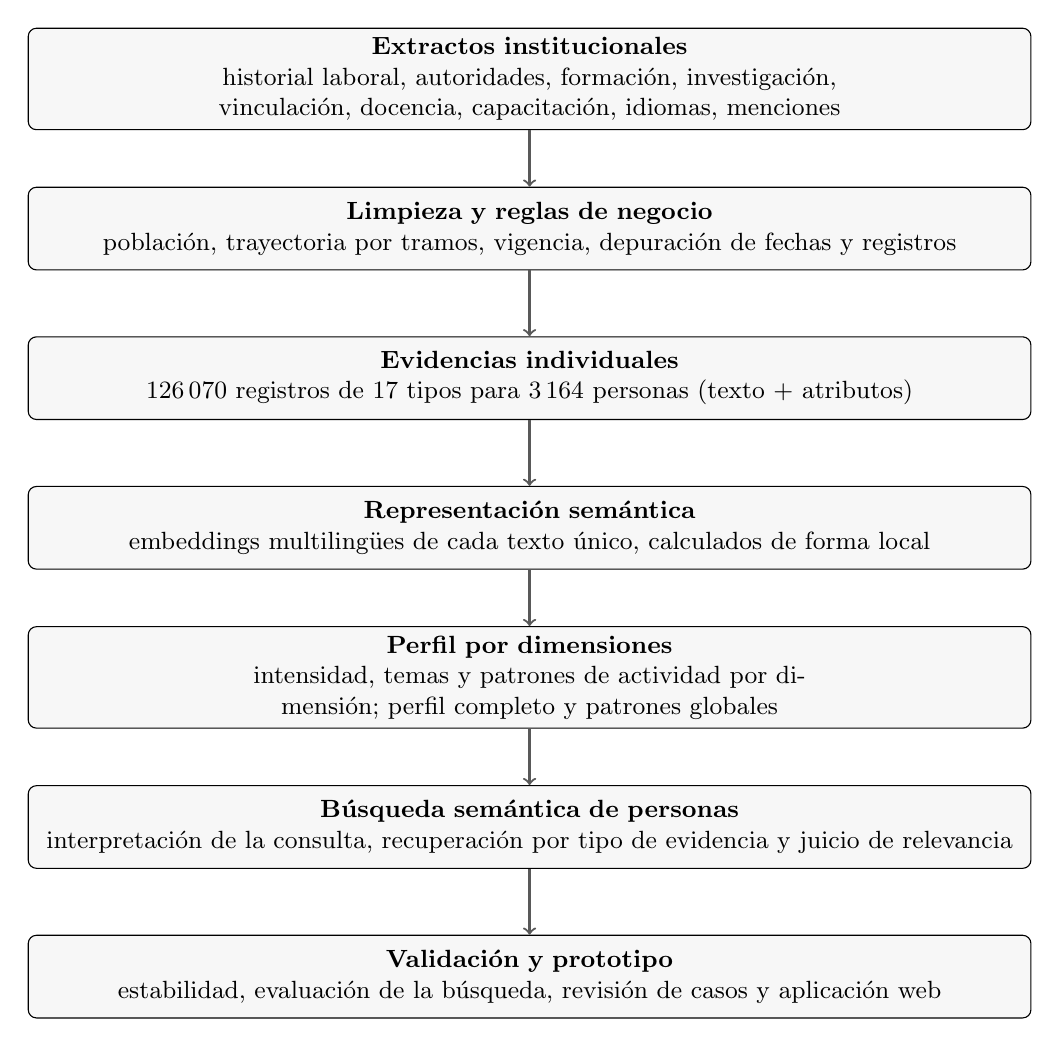
\begin{tikzpicture}[
        caja/.style={draw, rounded corners=3pt, align=center, text width=12.5cm, minimum height=1.05cm, font=\small, fill=gray!6},
        flecha/.style={->, thick, gray!70!black}]
        \node[caja] (f1) at (0,0)     {\textbf{Extractos institucionales}\\ historial laboral, autoridades, formación, investigación, vinculación, docencia, capacitación, idiomas, menciones};
        \node[caja] (f2) at (0,-1.9)  {\textbf{Limpieza y reglas de negocio}\\ población, trayectoria por tramos, vigencia, depuración de fechas y registros};
        \node[caja] (f3) at (0,-3.8)  {\textbf{Evidencias individuales}\\ 126\,070 registros de 17 tipos para 3\,164 personas (texto + atributos)};
        \node[caja] (f4) at (0,-5.7)  {\textbf{Representación semántica}\\ embeddings multilingües de cada texto único, calculados de forma local};
        \node[caja] (f5) at (0,-7.6)  {\textbf{Perfil por dimensiones}\\ intensidad, temas y patrones de actividad por dimensión; perfil completo y patrones globales};
        \node[caja] (f6) at (0,-9.5)  {\textbf{Búsqueda semántica de personas}\\ interpretación de la consulta, recuperación por tipo de evidencia y juicio de relevancia};
        \node[caja] (f7) at (0,-11.4) {\textbf{Validación y prototipo}\\ estabilidad, evaluación de la búsqueda, revisión de casos y aplicación web};
        \draw[flecha] (f1.south) -- (f2.north);
        \draw[flecha] (f2.south) -- (f3.north);
        \draw[flecha] (f3.south) -- (f4.north);
        \draw[flecha] (f4.south) -- (f5.north);
        \draw[flecha] (f5.south) -- (f6.north);
        \draw[flecha] (f6.south) -- (f7.north);
    \end{tikzpicture}
    \label{fig:flujo_general}
\end{figure}

Un aspecto que se cuidó durante todo el proyecto fue dejar constancia de cada decisión. Muchas reglas no se podían deducir de la documentación de los sistemas: qué significa un estado de contrato, cuándo una persona sigue trabajando en la institución o si una coordinación es un cargo o una tarea puntual. Cuando surgía una duda de este tipo, primero se medía su efecto sobre los datos reales y después se tomaba la decisión con quien conoce el negocio, sin suponer el significado de una columna. Cada decisión se anotó en un registro con el problema observado, las alternativas consideradas y el impacto medido. Al momento de escribir este documento el registro contiene más de cincuenta entradas, y buena parte de lo que se explica en las secciones siguientes proviene de él.

\section{Fuentes de datos}

\subsection{Extractos institucionales}

La información se obtuvo como extractos en formato CSV de los sistemas de Talento Humano, académicos y de investigación de ESPOL. La Tabla \ref{tab:fuentes} resume qué aporta cada uno. Cada extracto tiene su propio cuaderno de limpieza, de manera que los problemas de una fuente se resuelven en un solo lugar.

\begin{table}[!htbp]
    \centering
    \caption{Extractos institucionales utilizados y su aporte al perfil.}
    \label{tab:fuentes}
    \small
    \begin{tabular}{p{4.6cm} p{10.2cm}}
        \toprule
        \textbf{Extracto} & \textbf{Información que aporta} \\
        \midrule
        Datos personales & Personas contratadas o vigentes en los últimos cinco años; define la población. \\
        Historial laboral & Contratos, cargos, unidades, tipo de empleado, estados y fechas; base de la trayectoria y de la vigencia. \\
        Registro de autoridades & Designaciones de autoridades, coordinaciones y subrogaciones, con las siglas oficiales de cada unidad. \\
        Experiencia externa & Cargos e instituciones fuera de ESPOL, con país y fechas. \\
        Titulaciones & Títulos obtenidos y en curso, institución, país y áreas de conocimiento (CINE y Frascati). \\
        Proyectos de investigación & Proyectos, rol de cada participante, unidad, financiamiento y áreas. \\
        Proyectos de vinculación & Proyectos y programas con la comunidad y el rol en cada uno. \\
        Publicaciones & Artículos y otras publicaciones, medio, indexación y cuartil. \\
        Proyectos de grado & Tesis dirigidas, con nivel, programa y estudiantes. \\
        Ponentes & Participación como ponente en eventos académicos. \\
        Capacitaciones y certificados & Cursos, talleres, seminarios y certificaciones profesionales, con horas, modalidad y entidad. \\
        Idiomas & Idiomas declarados y su nivel, junto con el catálogo de idiomas. \\
        Menciones de honor & Premios y menciones recibidos. \\
        Carga académica & Cuatro extractos solapados de materias dictadas entre 1999 y 2026. \\
        Carga politécnica & Horas asignadas a docencia, investigación, vinculación y gestión desde 2013, con su catálogo de actividades. \\
        \bottomrule
    \end{tabular}
\end{table}

También se recibió un extracto de la heteroevaluación docente, que en esta versión no se incorporó al perfil. Además, se usó una lista de personas identificadas en defunción, cuyo único fin es excluirlas del análisis.

\subsection{Población de estudio}

La población se define como el personal docente y administrativo que estuvo contratado o vigente en algún momento de los últimos cinco años. Esa ventana delimita a quiénes se estudia, pero no recorta su historia: si una persona tiene registros anteriores, como materias dictadas en 2005 o un cargo de 2010, se conservan. De lo contrario, quien lleva veinte años en la institución aparecería con un perfil tan corto como el de alguien que ingresó hace poco.

La Tabla \ref{tab:poblacion} muestra cómo se llegó a la población final. Las personas identificadas en defunción se excluyen al definir la población, y todas las etapas posteriores heredan ese filtro. Durante el proyecto se detectó que, al regenerar los datos en un equipo donde faltaba la lista de defunciones, esas personas volvían a entrar sin ningún aviso. Para que no ocurra de nuevo, el proceso ahora se detiene si el archivo no está presente y una validación comprueba que ninguna evidencia pertenezca a una persona de esa lista.

\begin{table}[!htbp]
    \centering
    \caption{Definición de la población de estudio.}
    \label{tab:poblacion}
    \small
    \begin{tabular}{p{10cm} r}
        \toprule
        \textbf{Paso} & \textbf{Personas} \\
        \midrule
        Contratadas o vigentes en los últimos cinco años & 3\,195 \\
        Identificadas en defunción (excluidas) & $-24$ \\
        Sin ningún registro de trayectoria (excluidas) & $-7$ \\
        \midrule
        \textbf{Población de trabajo} & \textbf{3\,164} \\
        \bottomrule
    \end{tabular}
\end{table}

El análisis se repite en tres ámbitos independientes: todo el personal (3\,164 personas), el personal administrativo (1\,299) y el personal docente (1\,881). Los cálculos de cada ámbito no se mezclan, de modo que un percentil o un patrón docente se interpreta solo frente a otros docentes. El tipo de empleado se toma de los contratos activos hoy y no del último registro, porque algunas personas tienen a la vez un contrato administrativo y uno docente; un caso típico es quien dirige una unidad administrativa y dicta clases a tiempo parcial. Esas personas, 16 en la población, aparecen en ambos ámbitos.

\subsection{Tratamiento de la información personal}

Los extractos contienen datos personales, por lo que su manejo se ajustó a la Ley Orgánica de Protección de Datos Personales \parencite{LOPDP2021} y a criterios de minimización. Todo el procesamiento se realiza en equipos locales. Los modelos de embeddings y de reordenamiento se ejecutan en esos equipos, sin enviar textos institucionales a servicios externos. El único servicio externo es el modelo de lenguaje que interpreta las consultas del buscador, y a ese modelo solo llega el texto que escribe el usuario junto con un catálogo de tipos de evidencia ilustrado con ejemplos inventados; nunca recibe información de una persona.

El sexo y la edad no forman parte de ningún modelo ni se ofrecen como filtro. Los identificadores internos no se muestran en la interfaz ni en los enlaces. Los nombres de las personas se leen del extracto original en el momento de la consulta y no se copian a los resultados del modelo. Los resultados intermedios, que sí contienen identificadores, se mantienen fuera del repositorio de código.

\section{Preprocesamiento y reglas de negocio}

\subsection{Limpieza de cada fuente}

Los problemas encontrados fueron muy variados y, en su mayoría, propios de sistemas que llevan décadas en uso. Hubo fechas con errores de digitación, como una fecha de desvinculación del año 216 que producía una antigüedad negativa de casi mil años; desde entonces se rechaza cualquier año fuera del intervalo entre 1950 y dos años después del actual. También se encontró que la fecha de desvinculación, usada para cerrar un contrato, a veces caía después del fin pactado y lo alargaba: 501 contratos se extendían una mediana de 273 días por esta causa. Se fijó que la desvinculación solo cuenta cuando cae dentro del contrato y que nunca lo prolonga.

En la experiencia externa se eliminaron registros sin cargo, con textos de relleno, sin fecha de inicio, anteriores al nacimiento de la persona o duplicados, y se fusionaron los registros del mismo cargo e institución que se solapaban. En la carga académica se consolidaron tres extractos que repetían los mismos cursos, se definió que antes de 2015 se toman todos los registros (el sistema anterior solo guardaba cursos aprobados) y se asignó el nombre de la facultad actual a unidades que ya no existen; por ejemplo, los antiguos institutos de Ciencias Matemáticas, Física y Química pasan a FCNM. Algunos textos traen caracteres dañados por problemas de codificación del sistema de origen. Se comprobó que no los introduce el procesamiento y que solo se pueden recuperar con una nueva extracción, así que se mantienen tal como llegan.

\subsection{Reconstrucción de la trayectoria laboral}

El historial laboral registra contratos, no cargos. Una misma persona puede acumular decenas de contratos consecutivos para el mismo puesto, contratos cortos superpuestos y actos administrativos de pocos días. Para obtener una trayectoria legible se construyeron \textit{tramos}: periodos continuos en un mismo cargo y unidad. Se toleran recesos de hasta 90 días entre contratos de un cargo estructural y de hasta 60 días entre contratos puntuales, este último para absorber las vacaciones entre periodos académicos.

Los cargos se clasificaron con una taxonomía basada en reglas de texto sobre el nombre del cargo, con 11 categorías para el personal docente y 13 para el administrativo. Las reglas de cada rama se evalúan por separado para evitar confusiones por subcadenas; ``DIRECTOR'', por ejemplo, contiene la palabra ``RECTOR''. Los rótulos anteriores a la reforma de la LOES, como ``Profesor Principal'' o ``Profesor Agregado'', se unificaron con sus equivalentes actuales después de verificar que entre el 95\,\% y el 100\,\% de quienes los tuvieron aparecen más tarde con el cargo de titular correspondiente.

Hubo que resolver además tres situaciones que generaban cambios de cargo inexistentes. La primera fueron los contratos puntuales de servicios profesionales, tribunales o actividades académicas específicas, que conviven con el cargo estable de la persona. Al incluirlos en la secuencia de cargos se obtenían 11\,854 transiciones, con una persona que llegaba a 103; al tratarlos como eventos aparte, las transiciones bajaron a 4\,468. La segunda fueron los roles simultáneos, como el de un profesor titular que fue decano durante un periodo sin dejar de ser profesor. En 510 personas había tramos de distinta categoría superpuestos; se decidió que la línea principal la ocupe el tramo de mayor duración y que el otro se muestre como rol adicional. La tercera fueron las subrogaciones, que nunca se consideran un cambio de cargo, sin importar cuánto duren.

\subsection{Determinación de la vigencia}

Saber si una persona trabaja hoy en ESPOL resultó más difícil de lo esperado y fue la regla que más veces se corrigió. La primera versión consideraba vigente un contrato sin fecha de fin, pero el área de Talento Humano suele registrar una fecha planificada incluso en contratos activos, y algunos contratos activos tenían esa fecha ya vencida por retrasos en la renovación. Luego se tomó el estado del contrato como criterio principal, pero los movimientos administrativos cortos, que se registran en la misma tabla con una mediana de tres días de duración, cerraban contratos que en realidad seguían activos. También ocurría que encargos de uno o dos días del mismo cargo cerraban nombramientos abiertos, lo que dejaba fuera, entre otros, a la máxima autoridad de la institución.

La regla vigente reúne lo aprendido en esas correcciones:

\begin{itemize}
    \item La vinculación se calcula solo con los registros de tipo vinculación; los movimientos cortos no abren ni cierran periodos.
    \item Un registro finalizado posterior no cierra un nombramiento abierto si corresponde al mismo cargo.
    \item Un contrato activo hoy mantiene la vigencia aunque existan registros posteriores ya finalizados. Se entiende por activo un contrato en estado activo o por ejecutarse, ya iniciado, sin desvinculación pasada y con fecha de fin futura. Si no tiene fecha de fin, se exige además que la persona tenga algún registro en los últimos doce meses, para no revivir nombramientos antiguos que nunca se cerraron en el sistema.
\end{itemize}

Se consideró dar un margen de gracia de 30 a 60 días después del último contrato para cubrir renovaciones que aún no se registran, pero se descartó: la vigencia debe reflejar lo que dice el dato hoy y no una renovación que nadie ha confirmado. Con estas reglas el número de personas vigentes en el historial pasó de 850 en la primera versión a 1\,737. La vigencia no entra en ningún modelo; solo sirve para filtrar listas y resultados en el prototipo.

\section{Representación del perfil mediante evidencias}

\subsection{La evidencia como unidad de análisis}

En una primera etapa cada persona se describía con una fila de variables agregadas: años de servicio, número de publicaciones, nivel de formación y otras similares. Esa representación perdía justamente lo que interesa a quien busca a alguien para una comisión o un proyecto, que es \textit{de qué} trata su experiencia. Saber que una persona tiene doce publicaciones no dice si son de acuicultura o de redes eléctricas.

Por eso se adoptó como unidad la \textit{evidencia}: un elemento concreto y verificable del perfil, como un cargo, un título, un proyecto, una materia dictada o una certificación. Todas las evidencias siguen el mismo esquema, compuesto por un identificador, la persona, el tipo de evidencia, un texto y un conjunto de atributos. El texto es una descripción breve pensada para el análisis semántico. No incluye verbos como ``ocupó'' o ``fue'', fechas, identificadores ni el nombre de la institución, que aparecería en casi todas y no distingue a nadie. Un cargo, por ejemplo, se escribe como \textit{``Profesor titular auxiliar 1, Facultad de Ciencias Naturales y Matemáticas (FCNM)''}. Los atributos guardan en formato estructurado lo que no debe influir en la semántica: fechas, roles, niveles, cuartiles, horas o país.

El identificador de cada evidencia se obtiene de un \textit{hash} de su contenido, por lo que no cambia entre ejecuciones. Cada evidencia conserva una referencia a la fila de origen, de manera que cualquier dato mostrado en el prototipo puede rastrearse hasta el extracto.

\subsection{Tipos de evidencia}

Se definieron 17 tipos de evidencia agrupados en siete secciones. La Tabla \ref{tab:evidencias} presenta el número de evidencias y de personas de cada tipo en la versión actual. En total hay 126\,070 evidencias.

\begin{table}[!htbp]
    \centering
    \caption{Tipos de evidencia, número de evidencias y personas con al menos una.}
    \label{tab:evidencias}
    \small
    \begin{tabular}{p{3.2cm} p{6.6cm} r r}
        \toprule
        \textbf{Sección} & \textbf{Tipo de evidencia} & \textbf{Evidencias} & \textbf{Personas} \\
        \midrule
        \multirow{4}{*}{Trayectoria} & Cargo estructural en ESPOL & 5\,384 & 2\,454 \\
         & Contrato puntual en ESPOL & 3\,759 & 1\,932 \\
         & Función adicional o subrogación & 1\,214 & 601 \\
         & Experiencia externa & 7\,994 & 2\,481 \\
        \midrule
        \multirow{2}{*}{Formación} & Título obtenido & 6\,181 & 3\,138 \\
         & Formación en curso & 408 & 388 \\
        \midrule
        \multirow{5}{*}{Investigación} & Proyecto de investigación & 6\,373 & 1\,186 \\
         & Proyecto de vinculación & 2\,479 & 418 \\
         & Publicación & 7\,797 & 923 \\
         & Tesis dirigida & 4\,626 & 549 \\
         & Ponencia & 909 & 392 \\
        \midrule
        \multirow{2}{*}{Capacitación} & Capacitación & 42\,348 & 2\,566 \\
         & Certificación & 3\,733 & 1\,359 \\
        \midrule
        Idiomas & Idioma & 2\,594 & 2\,002 \\
        Reconocimientos & Mención de honor & 3\,291 & 1\,067 \\
        \midrule
        \multirow{2}{*}{Docencia} & Materia dictada & 10\,236 & 1\,257 \\
         & Actividad de carga politécnica & 16\,744 & 1\,621 \\
        \midrule
        \multicolumn{2}{l}{\textbf{Total}} & \textbf{126\,070} & \textbf{3\,164} \\
        \bottomrule
    \end{tabular}
\end{table}

\subsection{Reglas de construcción}

Cada tipo tiene sus propias reglas, documentadas junto al código, pero hay criterios que se repiten. El más importante es la agrupación: una evidencia representa un ítem y no un registro. Si una persona aparece en varios registros del mismo proyecto o tomó dos veces el mismo curso, se genera una sola evidencia y las repeticiones quedan en los atributos como periodos o participaciones. Los nombres se agrupan cuando son casi idénticos, tolerando diferencias de escritura, pero no se fusionan instituciones distintas con nombres parecidos, como ESPOL y ESPE.

Para agrupar fue necesario distinguir cuándo un número cambia el contenido y cuándo solo indica una edición. ``Cálculo I'' y ``Cálculo II'' son materias diferentes y no se unen; en cambio, la ``XV edición'' de un congreso y su edición de 2019 corresponden al mismo evento. Ante la duda, el número se trata como parte del contenido.

Algunos registros no se consideran evidencia porque no aportan información sobre la persona. Es el caso de los cursos institucionales obligatorios sin contenido temático, como las inducciones; de las tesis registradas con títulos genéricos del tipo ``Examen complexivo, fase 2''; de los certificados de asistencia cargados como ponencias y de los cargos de un solo día que no son subrogaciones. Tampoco son evidencia los registros con fecha de inicio futura. Nada de esto se borra en silencio: cada sección genera un archivo con los registros no considerados y el motivo, y una batería de validaciones automáticas revisa duplicados, fechas, personas fuera de la población y personas en defunción antes de guardar los resultados.

\section{Representación semántica del texto}

Para comparar evidencias por su significado, cada texto se transformó en un vector numérico (\textit{embedding}) con el modelo BGE-M3 \parencite{Chen2024}. Se eligió por ser multilingüe, un requisito práctico porque muchos títulos de publicaciones y proyectos están en inglés y el resto del perfil en español, y porque puede ejecutarse localmente con una GPU, lo que evita enviar textos institucionales a un servicio externo. Cada vector tiene 1\,024 dimensiones y se normaliza a longitud uno, de modo que el producto interno entre dos vectores equivale a su similitud coseno.

Como muchas evidencias se repiten entre personas (un proyecto con 32 participantes produce 32 evidencias con el mismo texto), solo se procesan los textos únicos, que son 87\,166. Los vectores se almacenan identificados por un \textit{hash} del texto, así que una ejecución posterior solo calcula los textos nuevos.

Se generaron dos versiones del texto. La completa se usa en la búsqueda y combina el contenido con su contexto, por ejemplo la unidad o el país. La versión \textit{de tema} conserva solo el título o nombre del ítem y se usa para descubrir temas. La separación se hizo después de observar que, con el texto completo, los metadatos y el idioma dividían temas que eran el mismo: los proyectos sobre ``banano'' y los de ``banana'' quedaban en grupos distintos.

En las pruebas apareció una limitación del modelo que conviene mencionar. El modelo no conoce las siglas institucionales: la similitud entre ``GTSI'' y el nombre completo de esa unidad era igual a la que se obtiene entre textos sin relación. La solución fue escribir en el texto la sigla y el nombre completo juntos, tomando la correspondencia del registro oficial de autoridades, en lugar de esperar que el modelo la infiriera.

\section{Evolución del enfoque de modelado}

Antes de llegar al modelo actual se probaron tres enfoques. Se resumen aquí porque explican varias decisiones del diseño final.

El primero fue el previsto en la propuesta: K-means sobre una tabla de variables estructuradas por persona. Los grupos resultantes reproducían en gran medida la división entre personal docente y administrativo y las categorías de cargo ya existentes, lo cual no aporta información nueva. Al revisar el modelo se encontró además un problema de circularidad: entre las variables de entrada estaban la propia categoría de cargo y otras que registraban eventos de la trayectoria, como haber pasado de administrativo a docente, de modo que el modelo ``descubría'' lo que ya se le había entregado. Se retiraron 22 variables por este motivo.

El segundo enfoque representó a cada persona con un único documento de texto que narraba toda su trayectoria, convertido en un solo vector. Al promediar todo en un vector, la fuente más abundante, que era capacitación, terminaba dominando el perfil, y las consultas sobre temas puntuales perdían precisión.

El tercero ya trabajó sobre las evidencias. Se construyeron tres vistas de cada persona: una semántica de trayectoria y gestión, otra semántica académica y una estructurada de 42 variables. Las tres se integraron con \textit{Similarity Network Fusion} \parencite{Wang2014}, un método que construye una red de similitud por vista y las fusiona por difusión sin concatenar variables de escalas distintas. Sobre la red fusionada se aplicó agrupamiento espectral. Los grupos fueron muy estables, con valores de ARI entre 0.84 y 0.99, pero demasiado gruesos: en el ámbito docente el criterio de selección eligió cuatro grupos y uno de ellos reunía a 1\,106 personas. Agregar un segundo nivel de subgrupos mejoró la resolución, aunque persistía un problema de fondo: como cada grupo mezclaba investigación, docencia, trayectoria y capacitación en una sola similitud, era difícil explicar a un usuario por qué dos personas quedaban juntas. Con esa experiencia se decidió reorganizar el perfil por dimensiones explícitas, como se describe a continuación. El cálculo multivista se conserva en el código como referencia, pero no forma parte del prototipo.

\section{Modelo de perfilamiento por dimensiones}

El modelo actual separa dos niveles. En el primero, el perfil se organiza en dimensiones fijas definidas por el tipo de evidencia; estas dimensiones no se descubren, se declaran. En el segundo, dentro de cada dimensión se buscan en los datos los temas y las formas de participación, sin fijar de antemano roles, temas ni número de grupos. Finalmente, todas las dimensiones se combinan en un perfil completo sobre el que se buscan patrones globales. Todo el proceso se ejecuta por separado en cada ámbito.

\subsection{Dimensiones del perfil}

Se definieron doce dimensiones. La Tabla \ref{tab:dimensiones} muestra los tipos de evidencia que alimentan cada una y los componentes con que se mide. Trayectoria se dividió en dos dimensiones, una dentro de ESPOL y otra externa, porque responden a preguntas distintas: cuánto conoce alguien la institución y qué experiencia trae de fuera.

\begin{table}[!htbp]
    \centering
    \caption{Dimensiones del perfil y componentes utilizados para medir su intensidad.}
    \label{tab:dimensiones}
    \small
    \begin{tabular}{p{3.1cm} p{4.3cm} p{7.3cm}}
        \toprule
        \textbf{Dimensión} & \textbf{Evidencias} & \textbf{Componentes} \\
        \midrule
        Investigación & Proyectos de investigación, publicaciones & Proyectos, proyectos dirigidos o codirigidos, publicaciones, publicaciones en Q1--Q2 \\
        Ponencias & Ponencias & Ponencias, ponencias en el exterior \\
        Vinculación & Proyectos de vinculación & Proyectos, proyectos o programas dirigidos, años en vinculación \\
        Tesis dirigidas & Tesis dirigidas & Tesis, estudiantes dirigidos, tesis de maestría de investigación o doctorado \\
        Docencia & Materias, carga politécnica & Materias, semestres con docencia, estudiantes atendidos, horas de carga en docencia \\
        Formación & Títulos, formación en curso & Nivel máximo (peso doble), posgrados, título del exterior, posgrado en curso (medio peso) \\
        Capacitación & Capacitaciones & Cursos, horas, cursos en el exterior \\
        Certificaciones & Certificaciones & Certificaciones, certificaciones vigentes, horas \\
        Idiomas & Idiomas & Idiomas extranjeros, nivel máximo en un idioma extranjero \\
        Reconocimientos & Menciones de honor & Menciones, menciones del exterior \\
        Trayectoria en ESPOL & Cargos, contratos puntuales, funciones adicionales & Años en cargos estructurales, número de cargos y contratos, funciones adicionales \\
        Experiencia externa & Experiencia externa & Años, experiencias, experiencias en el exterior, experiencias académicas \\
        \bottomrule
    \end{tabular}
\end{table}

\subsection{Intensidad por dimensión}

Para cada persona $p$ y dimensión $d$ se calcula una intensidad entre 0 y 100. Primero se obtienen los componentes $c_{pj}$ a partir de los atributos de sus evidencias. Los conteos y los años se transforman con $\log(1+x)$, de manera que pasar de cero a cinco publicaciones pese más que pasar de cien a ciento cinco. Cada componente se divide entre su máximo en el ámbito y se combina en un índice bruto:

\begin{equation}
    I_{pd} = \frac{\sum_{j \in d} w_j \, \dfrac{c_{pj}}{\max_{q} c_{qj}}}{\sum_{j \in d} w_j},
\end{equation}

donde los pesos $w_j$ son iguales salvo en Formación, en la que el nivel máximo pesa el doble y el posgrado en curso la mitad. La intensidad es el percentil del índice dentro del ámbito:

\begin{equation}
    \text{Int}_{pd} = 100 \cdot \frac{\left|\{\, q : I_{qd} \le I_{pd} \,\}\right|}{n},
\end{equation}

con $n$ igual al número de personas del ámbito. Quien no tiene evidencias de la dimensión recibe intensidad cero, y no un percentil compartido con las demás personas sin registros.

Hay tres aspectos de esta medida que se deben tener presentes al leerla. Las dimensiones son independientes y no suman 100, porque se trata de intensidades y no de una composición del perfil. El percentil es relativo al ámbito: un 80 en Investigación entre administrativos no equivale a un 80 entre docentes. Por último, lo que se mide es la intensidad de la evidencia registrada en los sistemas, no la capacidad de la persona. Para que el número sea explicable, se guarda el aporte de cada componente al índice, y la interfaz muestra de dónde sale cada valor.

\subsection{Temas dentro de cada dimensión}

Los temas responden a la pregunta \textit{de qué trata} la evidencia de una persona en una dimensión. Se agrupan las evidencias, no las personas, porque una persona suele trabajar en varios temas. En una prueba en la que se promediaron los vectores de cada persona antes de agrupar, los temas resultantes se describían con términos tan generales como ``Ecuador, desarrollo, estudio''.

El procedimiento sigue la lógica de BERTopic \parencite{Grootendorst2022}. Los vectores del texto de tema se reducen a cinco dimensiones con UMAP \parencite{McInnes2018}, usando distancia coseno y 15 vecinos, y se agrupan con HDBSCAN \parencite{Campello2013}. HDBSCAN no requiere fijar el número de grupos y deja sin asignar los textos que no pertenecen claramente a ninguno; el tamaño mínimo de un tema se fijó en el 0.5\,\% de los textos de la dimensión, con un mínimo de diez. Los textos no asignados se adjudican al tema de centroide más cercano y quedan marcados como asignados por cercanía, ya que en dimensiones como Investigación representan cerca de un tercio de los textos. Cada tema se describe con sus términos más distintivos, obtenidos con c-TF-IDF, y con sus ejemplos más frecuentes. Para cada persona se calcula la proporción de sus evidencias de la dimensión que cae en cada tema.

Idiomas no tiene temas, porque sus evidencias no tienen contenido temático. Tampoco se buscan temas en una dimensión con menos de 40 personas con evidencias o menos de 60 textos, situación que se da, por ejemplo, en Vinculación dentro del ámbito administrativo.

\subsection{Patrones de actividad dentro de cada dimensión}

Los patrones de actividad responden a una pregunta distinta: \textit{cómo} participa la persona en la dimensión. Dos investigadores pueden tener el mismo número de publicaciones y, sin embargo, uno dirigir sus proyectos y publicar en revistas de primer cuartil mientras el otro participa como coautor en proyectos ajenos.

Para capturar esa diferencia, a los componentes de la dimensión se agregaron proporciones que no dependen del volumen: la parte de los proyectos que la persona dirige, la parte de sus publicaciones en Q1--Q2 o como autor principal, la proporción de capacitaciones en el exterior, las horas por curso o los estudiantes por materia, entre otras. Estas variables se estandarizan entre quienes tienen evidencias de la dimensión y se agrupan con K-means \parencite{Lloyd1982}. El número de grupos se elige entre 3 y 6 según el mayor coeficiente de silueta \parencite{Rousseeuw1987}, con la condición de que ningún grupo tenga menos del 3\,\% de las personas.

Antes de llegar a esta configuración se probó el agrupamiento espectral y se probó también agrupar sin las proporciones. En ambos casos los patrones solo separaban a las personas por volumen de actividad y aparecía un grupo ``típico'' con cerca del 75\,\% de las personas. Con K-means y las proporciones emergieron formas de participación reconocibles; en la dimensión de Investigación de los docentes, por ejemplo, se distinguen quienes dirigen sus proyectos, quienes son muy activos en todos los componentes, quienes publican sobre todo en revistas Q1--Q2, quienes son autores principales con poco volumen y quienes tienen una participación baja.

Además del patrón asignado, cada persona recibe una afinidad con todos los patrones de la dimensión, calculada a partir de la distancia $d_{pk}$ al centroide de cada patrón $k$:

\begin{equation}
    a_{pk} = \frac{1/d_{pk}^{2}}{\sum_{l} 1/d_{pl}^{2}}.
\end{equation}

Las afinidades suman uno, pero no son probabilidades; indican cercanía relativa. Como representante de cada patrón se elige a la persona vigente más cercana a su centroide, de modo que siempre sea alguien que hoy trabaja en la institución.

\subsection{Perfil completo y patrones globales}

Las dimensiones por separado no permiten ver a la persona en conjunto, por ejemplo a quien combina investigación intensa con muchos reconocimientos. Para eso se construye un vector de perfil por persona y ámbito. Por cada dimensión con patrones, el bloque correspondiente son las afinidades de la persona con esos patrones multiplicadas por su intensidad dividida entre 100. En las dimensiones sin patrones el bloque es solo la intensidad dividida entre 100. Cada bloque recoge entonces cuánto (la magnitud) y cómo (la dirección), y las doce dimensiones pesan lo mismo. Los temas no se incluyen en este vector, ya que el contenido se atiende mejor con la búsqueda semántica descrita más adelante.

Sobre ese vector se aplicó K-means para descubrir patrones globales. El número de patrones se eligió entre 4 y 8 con un criterio en dos pasos: primero se descartaron los valores de $k$ cuya estabilidad, medida con el índice de Rand ajustado (ARI) \parencite{Hubert1985} entre la partición completa y particiones sobre submuestras del 90\,\%, fuera menor que 0.9; entre los restantes se eligió el de mayor silueta. Una persona se marca como de perfil mixto cuando su segunda afinidad alcanza al menos el 80\,\% de la primera.

Los patrones globales con 60 personas o más se dividen en microarquetipos con el mismo método, ahora con $k$ entre 2 y 5. Cada microarquetipo se describe frente a su patrón global y no frente a todo el ámbito; cuando no se distingue de él, la descripción lo indica de forma explícita. Para ordenar a los integrantes de un grupo se calcula su similitud con el representante:

\begin{equation}
    s_p = 1 - \frac{d(p, r)}{\max_{q \in G} d(q, r)},
\end{equation}

donde $r$ es el representante y $G$ el grupo. Vale 100\,\% para el representante y 0\,\% para el integrante más distinto a él. Es una medida relativa al grupo y no debe compararse entre grupos.

La descripción de cada patrón se genera solo con hechos medidos. Se mencionan las dimensiones cuya intensidad media se aleja en 15 puntos o más de la del ámbito y los patrones por dimensión que distinguen al grupo, es decir, aquellos con un \textit{lift} de al menos 1.5 que abarcan al menos la mitad de quienes tienen evidencias y al menos el 30\,\% del grupo. Este segundo criterio se añadió porque, sin él, dos patrones del personal administrativo quedaban descritos de la misma forma aunque se diferenciaban en cómo participan. Los patrones llevan nombres neutrales (``Patrón global 1'', ``Patrón global 1.2''), por decisión expresa, para no presentar como categoría laboral algo que es una agrupación estadística.

El vector de perfil también se usa para dos funciones de exploración. La primera es un mapa en dos dimensiones obtenido con t-SNE \parencite{vanderMaaten2008}, que sirve solo para visualizar, pues los grupos no se calculan sobre ese plano. La segunda es la lista de las quince personas más cercanas en distancia euclidiana, que en la ficha de cada persona se muestra junto con las dimensiones que ambas comparten con intensidad alta.

\section{Búsqueda semántica de personas}

Los perfiles sirven para explorar, pero la necesidad más frecuente en los casos de uso es más concreta: encontrar a quien tenga experiencia en un tema para integrar una comisión o un equipo. Para eso se construyó un buscador que trabaja directamente sobre las evidencias y que no depende de los grupos. El proceso tiene cuatro etapas.

\textbf{Interpretación de la consulta.} El usuario escribe en lenguaje natural, por ejemplo ``alguien con doctorado y al menos cinco años de experiencia docente en estadística''. Un modelo de lenguaje (\textit{gpt-oss-120b}, a través del servicio Groq) descompone la consulta en capacidades. A cada una le asigna un tema, una importancia (obligatoria o deseable), los tipos de evidencia en que podría acreditarse y una reformulación en el estilo de cada tipo. Además extrae requisitos de la persona, como nivel de formación o idiomas, y requisitos de años. La respuesta se valida contra un esquema JSON estricto, se usa temperatura cero y se guarda en caché. Si el servicio no responde, la consulta completa se busca como una sola capacidad en todos los tipos.

\textbf{Recuperación por capacidad y tipo.} Primero se filtra el universo de personas por vigencia y por los requisitos personales. Luego, para cada capacidad y cada tipo de evidencia pertinente, se combinan dos búsquedas: una densa, con la similitud coseno entre los embeddings de la consulta y de las evidencias, y una léxica con BM25 \parencite{Robertson2009}, útil para siglas y nombres propios. Ambas listas se fusionan con \textit{Reciprocal Rank Fusion} \parencite{Cormack2009} con $k=60$, y los 40 mejores candidatos de cada tipo pasan a la etapa siguiente. Buscar por tipo evita que los tipos más numerosos, como capacitación, acaparen los resultados.

\textbf{Juicio de relevancia.} Un modelo de reordenamiento de tipo \textit{cross-encoder} (BGE-reranker-v2-m3) lee juntos el tema de la capacidad y el texto de cada evidencia candidata y estima su relevancia. Una capacidad se considera cubierta cuando la relevancia supera 0.3, umbral elegido mediante la evaluación descrita en la sección siguiente. El modelo compara solo el tema y no la descripción completa de la capacidad. Cuando se le pasaba la descripción completa, las palabras propias del tipo de actividad generaban falsos positivos: un proyecto sobre ``aprendizaje autónomo'' obtenía 0.97 frente a una consulta sobre ``proyectos de investigación en aprendizaje automático''.

\textbf{Ordenamiento de personas.} El puntaje de una persona en una capacidad es el de su mejor evidencia; tener muchas evidencias parecidas no suma, para no favorecer a quien simplemente tiene más registros. Los requisitos de años se verifican uniendo los intervalos de las evidencias relevantes, de modo que dos periodos simultáneos no se cuentan dos veces; si las fechas no alcanzan, el requisito figura como no verificable y no como incumplido. Las personas se ordenan por el número de capacidades obligatorias cubiertas, luego por la media geométrica de sus puntajes en ellas (una capacidad débil arrastra el total) y por último por las deseables.

El resultado se muestra con su justificación: qué entendió el sistema de la consulta, qué capacidades cubre cada persona y con qué evidencias, con su tipo y sus fechas. No se muestra la similitud coseno porque no es interpretable como porcentaje; en pruebas anteriores, consultas sin ninguna relación con los textos obtenían valores entre 0.70 y 0.86, casi iguales a los de consultas pertinentes. En su lugar se indica una relevancia alta, media o baja, y una nota fija recuerda que la ausencia de evidencia no equivale a la ausencia de una capacidad.

\section{Validación}

\subsection{Validación cuantitativa de los agrupamientos}

Para cada agrupamiento se calcularon dos medidas. La silueta \parencite{Rousseeuw1987} indica qué tan separados están los grupos. La estabilidad se midió como el ARI promedio entre la partición obtenida con todas las personas y las obtenidas al repetir el procedimiento sobre submuestras aleatorias del 90\,\%. En este tipo de datos la silueta resulta baja, entre 0.09 y 0.16 en los patrones globales, porque los perfiles cambian de forma gradual y no forman nubes separadas. Por eso se le dio más peso a la estabilidad y se exigió que la partición elegida tuviera un ARI de al menos 0.9; un ARI cercano a 1 significa que los grupos casi no cambian al retirar una parte de las personas. Se fijaron también tamaños mínimos de grupo para evitar patrones formados por unos pocos casos atípicos.

\subsection{Evaluación del buscador}

Como no existe un conjunto de consultas con respuestas conocidas, se construyó una evaluación de tipo \textit{known-item}. Se tomaron 80 textos de evidencias pertenecientes a entre una y tres personas, 40 títulos de publicaciones y 40 nombres de materias, que son información pública. Un modelo de lenguaje los parafraseó como los escribiría alguien que busca a esa persona; por ejemplo, ``Instalaciones industriales'' se convirtió en ``Buscamos experto en sistemas de instalaciones industriales''. Una consulta se considera acertada si la persona dueña de la evidencia aparece entre los primeros $k$ resultados, y se reportan \textit{recall@k} y el rango recíproco medio (MRR).

Con esta evaluación se compararon cinco variantes del buscador: búsqueda densa global como línea base, búsqueda híbrida global, y tres variantes con interpretación de la consulta y búsqueda por tipo que difieren en el criterio de relevancia (posición dentro del tipo, \textit{cross-encoder} o fusión de ambos). La variante con \textit{cross-encoder} fue la elegida, y con la misma evaluación se recorrió una grilla de umbrales de relevancia. Los resultados se presentan en el capítulo siguiente. Esta evaluación tiene un sesgo conocido: en consultas genéricas, como las de materias, puede haber muchas personas legítimamente relevantes además de la dueña de la evidencia, y la medida las cuenta como fallos.

\subsection{Pruebas de consistencia}

El código incluye pruebas automáticas que se ejecutan después de cada cambio. Comprueban, entre otras cosas, que las afinidades sean finitas, no negativas y sumen uno; que los cálculos de un ámbito no usen personas de otro; que los representantes sean personas vigentes y que ninguna evidencia corresponda a personas fuera de la población. Cada ejecución del modelo se guarda en una carpeta identificada con la fecha y una huella calculada sobre los archivos de entrada y los parámetros, lo que permite reproducir cualquier versión y saber si los resultados que muestra el prototipo están desactualizados frente a los datos.

\subsection{Validación cualitativa}

La revisión de casos concretos fue la forma más útil de encontrar errores. Varias de las correcciones de vigencia descritas antes surgieron al notar que personas que trabajan hoy en ESPOL, entre ellas autoridades, no aparecían en el prototipo. Del mismo modo se detectó que el cargo mostrado como actual a veces correspondía a un encargo de pocos días y no al puesto real de la persona. Esta revisión se ha hecho hasta ahora con conocimiento interno del funcionamiento de la institución. Queda pendiente la validación formal con responsables de Talento Humano y de las unidades académicas, que consistirá en revisar si los patrones son reconocibles y útiles para los casos de uso y en calificar los resultados del buscador para un conjunto de consultas reales con una escala de 0 a 2.

\subsection{Interpretabilidad}

En lugar de explicar después un modelo opaco, se optó por que cada resultado pueda explicarse desde su construcción. La intensidad de cada dimensión se descompone en el aporte de sus componentes. Cada patrón se describe con las diferencias medidas frente a su referencia y se ilustra con una persona real, su representante. En el buscador, cada persona aparece junto con las evidencias que justifican su posición. Con esto, quien consulta puede verificar por sí mismo por qué el sistema propone a alguien y descartar la sugerencia si no la considera adecuada.

\section{Prototipo}

El prototipo se diseñó pensando en su mantenimiento. Los cálculos pesados (embeddings, dimensiones, patrones e índices de búsqueda) se ejecutan fuera de línea y guardan sus resultados versionados. Una API desarrollada con FastAPI solo lee esos resultados y, al iniciar, compara la huella de la versión con la de los datos para advertir si es necesario recalcular. La interfaz se construyó con React y TypeScript, y el conjunto se empaqueta en contenedores Docker para facilitar su instalación en servidores de la institución.

La interfaz tiene tres vistas principales. La vista de perfiles muestra, para cada ámbito, las dimensiones con sus temas y patrones y el perfil completo con sus patrones globales, microarquetipos y el mapa de personas. La ficha de cada persona reúne su intensidad por dimensión, sus temas y patrones, su trayectoria laboral dibujada en una línea de tiempo y las personas con un perfil parecido. La vista de búsqueda permite escribir una consulta abierta y filtrar por vigencia, que es el único filtro disponible. La Tabla \ref{tab:herramientas} resume las herramientas utilizadas.

\begin{table}[!htbp]
    \centering
    \caption{Herramientas utilizadas en cada etapa.}
    \label{tab:herramientas}
    \small
    \begin{tabular}{p{4.2cm} p{10.6cm}}
        \toprule
        \textbf{Etapa} & \textbf{Herramientas} \\
        \midrule
        Limpieza e integración & Python, pandas, cuadernos Jupyter \\
        Representación semántica & BGE-M3 mediante \textit{sentence-transformers}, ejecutado en GPU \\
        Modelado & scikit-learn (K-means, silueta, ARI, t-SNE), UMAP, HDBSCAN \\
        Búsqueda & BGE-reranker-v2-m3, BM25 implementado con SciPy, modelo \textit{gpt-oss-120b} vía Groq, pydantic \\
        Prototipo & FastAPI, React, TypeScript, Docker \\
        Pruebas & pytest \\
        \bottomrule
    \end{tabular}
\end{table}

\section{Limitaciones de la metodología}

Algunas limitaciones afectan la lectura de los resultados y conviene declararlas desde ahora:

\begin{itemize}
    \item El archivo de población no incluye a todas las personas vigentes. De 1\,737 personas vigentes según el historial laboral, alrededor de 1\,360 tienen perfil; las demás están fuera del extracto de datos personales de los últimos cinco años. La causa se está revisando con la institución.
    \item El perfil refleja lo que está registrado en los sistemas. Una persona con poca información cargada aparecerá con baja intensidad aunque tenga experiencia que nunca se registró.
    \item Las intensidades y los patrones son relativos a cada ámbito y no deben compararse entre ámbitos.
    \item Algunas decisiones de negocio siguen abiertas, como el tratamiento de los contratos temporalmente inactivos o de los encargos cortos repetidos en la trayectoria.
    \item El servicio gratuito del modelo de lenguaje limita el número de consultas nuevas por día, y el umbral de relevancia del buscador se calibró con consultas de una sola capacidad.
    \item La validación con responsables institucionales todavía no se ha realizado.
\end{itemize}
